\documentclass[11pt]{report}
\usepackage[utf8]{inputenc}
\usepackage[T1]{fontenc}
\usepackage[unicode=true]{hyperref}
\usepackage{lmodern}
\usepackage[french]{babel}

%%% PAGE DIMENSIONS
\usepackage{geometry}
\geometry{a4paper}
\geometry{top=2.5cm, bottom=2.5cm, left=4.5cm , right=3.5cm}
\usepackage{graphicx}


%%% PACKAGES
\usepackage{booktabs} % for much better looking tables
\usepackage{array} % for better arrays (eg matrices) in maths
\usepackage{paralist} % very flexible & customisable lists (eg. enumerate/itemize, etc.)
\usepackage{verbatim} % adds environment for commenting out blocks of text & for better verbatim
\usepackage{subfig} % make it possible to include more than one captioned figure/table in a single float
\usepackage{amssymb,amsmath}
\usepackage{xcolor}
\usepackage{sistyle}
\usepackage{shorttoc}
\usepackage{titlesec}
\usepackage{titletoc}

\hypersetup{breaklinks=true,
            pdfauthor={Thibault Deutsch (deutsc\_t); Rémy Bernier (bernie\_r); Marc Fresne (fresne\_m); Anthony Belthier (belthi\_a)},
            pdftitle={Rapport de projet},
            colorlinks=true,
            citecolor=blue,
            urlcolor=blue,
            linkcolor=black,
            pdfborder={0 0 0}}

\setlength{\parskip}{6pt plus 2pt minus 1pt}
\setlength{\emergencystretch}{3em}  % prevent overfull lines

\setcounter{secnumdepth}{3}
\setcounter{tocdepth}{4}
\renewcommand{\thechapter}{\Roman{chapter}}
\renewcommand{\thesection}{\arabic{section}.}
\renewcommand{\thesubsection}{\arabic{section}.\arabic{subsection}}
\renewcommand{\thesubsubsection}{\arabic{section}.\arabic{subsection}.\arabic{subsubsection}}

\usepackage{fancyhdr} % This should be set AFTER setting up the page geometry
\pagestyle{fancy}
\fancyhead[L]{Emagine Studio}
\fancyhead[C]{}
\fancyhead[R]{Troma}

\title{Rapport de projet}
\author{Thibault Deutsch (deutsc\_t) \and Rémy Bernier (bernie\_r) \and Marc Fresne (fresne\_m) \and Anthony Belthier (belthi\_a)}
\date{12 juin 2014}

\dottedcontents{chapter}%
  [\dimexpr 10mm]
  {}
  {\dimexpr 10mm}
  {3.2mm}

\begin{document}
\renewcommand{\labelitemi}{$\bullet$}

\begin{titlepage}
\newcommand{\HRule}{\rule{\linewidth}{0.5mm}} % Defines a new command for the horizontal lines, change thickness here

%----------------------------------------------------------------------------------------
%	LOGO SECTION
%----------------------------------------------------------------------------------------
\flushright
\includegraphics[width = 4.5cm]{EPITA.png}\\[0.5cm] % Include a department/university logo - this will require the graphicx package

%----------------------------------------------------------------------------------------
%	HEADING SECTIONS
%----------------------------------------------------------------------------------------
\textsc{\Large Rapport de projet}\\[0.15cm] % Major heading such as course name
\textsc{\large 1\ier{} année du cycle préparatoire}\\[3cm] % Minor heading such as course title

%----------------------------------------------------------------------------------------
%	TITLE SECTION
%----------------------------------------------------------------------------------------
\center
\HRule \\[0.5cm]
{\Huge \bfseries Troma}\\[0.3cm] % Title of your document
\textsc{\Large Jeu vidéo en 3D}\\[0.1cm]
\large Réalisé par le groupe \emph{Emagine Studio}\\[1.5cm]
\large 12 juin 2014\\[0.1cm]
\HRule \\[2cm]

\includegraphics[width = 4cm]{eie.png}\\[1cm]

\Large
\textbf{Thibault Deutsch} (\emph{deutsc\_t}) \\
\textbf{Rémy Bernier} (\emph{bernie\_r}) \\
\textbf{Marc Fresne} (\emph{fresne\_m}) \\
\textbf{Anthony Belthier} (\emph{belthi\_a})\\[2cm]

%----------------------------------------------------------------------------------------
\vfill % Fill the rest of the page with whitespace

\end{titlepage}

\newpage
\pagenumbering{arabic}
\shorttableofcontents{Sommaire}{1}

\chapter*{Introduction}

Ce document est le rapport de la soutenance finale. Il a pour but de présenter une synthèse sur le travail fournit par l'équipe en charge du projet. Cette équipe est formée de quatre étudiants en première année du cycle préparatoire de l'EPITA : Anthony BELTIER (beltie\_a), Remy BERNIER (bernie\_r), Thibault DEUTSCH (deutsc\_t) et Marc FRESNE (fresne\_m).

Le projet consiste en la programmation d'un logiciel au choix en C\# ou en CAML. Le développement s'est déroulé sur une période d'environ 6 mois, découpée en 4 étapes : la remise d'un cahier des charges, d'une soutenance de présentation, d'une soutenance intermédiaire de démonstration des avancées et d'une soutenance finale pour présenter le projet achevé. Il a pour but l'apprentissage du développement, du travail de groupe, de la réponse à une demande précise dans un temps donné. L'objectif est d'offrir aux étudiants l'occasion de réaliser un projet dans des conditions similaires à celles qui régissent le monde professionnel.

Nous avons choisis de réalisé un jeu vidéo car c'est un domaine que nous apprécions et que nous pensions que cela faciliterait la réalisation par le côté ludique. Nous avons opté pour l’utilisation du C\# car il s’agit d’un langage particulièrement adapté à ce type de projet. 

Nous nous sommes orientés sur un jeu en 3D car cela représentait un véritable défi au vue de l'expérience du groupe. Nous avons retenus le style de jeu FPS (First Person Shooter) car nous apprécions ce type de jeu mais aussi 'car la demande dans l'industrie du jeu vidéo ne cesse de croitre. La thématique de notre jeu est celle de la seconde Guerre Mondiale par soucis d'originalité, en effet l'offre s’oriente aujourd'hui principalement vers des univers futuristes, mais aussi afin d'être en accord avec le 70\ieme anniversaire du débarquement.

Vous trouverez dans la suite de ce rapport une présentation générale du projet, une présentation détaillée sur les différentes dimensions du développement ainsi qu'une synthèse personnelle sur cette expérience.

\chapter{Modélisation}

Un jeu en 3D tel qu'un FPS se base sur un univers complet plus ou moins réaliste. Afin d'offrir un tel univers il est important de poser des bases indispensables à la conception et à la création de celui-ci. Dans un premier temps il faut choisir l’environnement ainsi que le contexte dans lequel se déroulera le jeu.

Nous avons choisis un thème historique : la seconde Guerre Mondiale. Cela implique donc de respecter un minimum le contexte ainsi que les décors pour rendre le jeu crédible et agréable à jouer. Par ailleurs notre jeu disposant de deux modes, un solo et un multijoueur, avec des objectifs relativement différents, nous avions un minimum de deux cartes à modéliser.  Toutes les modélisations ont été réalisées à l’aide du logiciel Blender et les textures à l’aide de Gimp.  Ces deux logiciels sont libres et gratuits.

\section{La conception}

La conception est l’étape de création d’une liste des objets à modéliser ainsi que d’élaboration des plans pour les différentes cartes et bâtiments. Comme indiqué dans l’introduction nous avions besoin de deux cartes, l’une destinée au mode solo, l’autre au mode multi-joueurs. La première sera évidemment plus petite que la deuxième mais aussi différentes d’un point de vue décors.

La carte solo prend place aux Etats-Unis dans un milieu rural. 

TODO: photo plan

La carte multi-joueurs prend place en Europe dans un milieu urbain. Elle est inspirée d’une partie de Cracovie, Pologne. Cependant pour des raisons de jouabilité nous avons modifié quelque peu sa structure. Voici un plan des bâtiments principaux répartis sur la carte.

TODO: photo plan2

La réalisation de plan tels que ceux-ci permet d’obtenir une liste précise des bâtiments a modélisé avec leur forme mais aussi leur dimension. 

TODO: partie sur l'heightmap

\section{Les techniques de modélisation}

Une fois la conception terminée, la modélisation peut commencer. Afin de ne pas trop alourdir le jeu et ainsi conserver de bonne performance, chaque objet soit être simplifié au maximum. En effet les objets sont formés à partir de ``vertices'' (sommets) plus leur nombre et grand plus le fichier est gros et plus les procédures de traitement de ce fichier sont longues.

\subsection{Les bâtiments}

Pour ce faire, chaque bâtiment a été réduit en deux parallélépipèdes, un carré ou rectangle pour les murs, et un trapézoïdal pour le toit. Ensuite il a suffi de modéliser différents modèles de porte ou de fenêtre et de les associer à ces bâtiments.

TODO: Figure mur + toit + fenêtre = bâtiment

Par ailleurs il est important que le ``mesh'' soit découpé en plusieurs ``objects''  si la partie au sol n’est pas strictement rectangulaire. En effet cela facilite énormément la gestion des collisions. Des explications plus détaillées seront fournies à la section correspondante.

TODO: Figure gare-quai

\subsection{Le personnages et les armes}

Pour des modèles aussi complexes il est encore plus important de maintenir le nombre de « vertices » aussi bas que possible. Une technique de modélisation pour y arriver et d’utiliser des formes rectangulaire afin d’obtenir une silhouette grossière de l’objet considérée puis d’utilisé des « modifiers » pour déformer le maillage et le rapprocher de la forme souhaitée. La réalisation de la silhouette est possible sans être un as du dessin en s’appuyant sur une image qu’il est possible d’avoir en arrière-plan. Cette technique s’appelle « blueprint » (en référence au plan de couleur bleu).

\section{Les textures}

Les textures sont de simples images utilisées pour « habiller » les modèles. Afin de pouvoir se servir de ses images sur un volume il est nécessaire d’avoir une sorte de patron. Cette étape a pour nom l’UV mapping et se décompose en 3 actes : l’édition des lignes de découpe, le dépliage et enfin la création de la texture en fonction du plan obtenu.

\subsection{Le découpage}

Cette étape n’est pas toujours indispensable, surtout pour des modèles très simples. Cependant elle permet de délimité avec certitude les différentes surfaces qui apparaitront sur la carte UV. Les lignes de découpe sont appelées ``seems'', pour les créer il faut simplement sélectionner les arrêtes  concernées. 

\begin{figure}[htbp]
\centering
\includegraphics[width=8cm]{seems.png}
\caption{Capture d'écran de blender montrant les ``seems''}
\end{figure}

\subsection{Le dépliage}

Il s’agit de la mise à plat des surfaces du volume selon des lignes de découpe, créées manuellement ou par l’ordinateur. Cette carte fait correspondre ses coordonnées U et V aux coordonnées dans l’espace X, Y et Z de chaque point. Il existe plusieurs options de dépliage qui ne seront pas abordées dans le rapport. En effet avec un découpage adéquat un dépliage classique offre de bon résultat. 

Une fois effectué on obtient donc le patron du modèle. Celui-ci est éditable depuis blender, c’est-à-dire que l’on peut modifier si besoin la position des différentes faces. Cela permet d’ajuster la position des différentes faces selon le résultat souhaité. Par ailleurs il est aussi possible de voir à quel point ont été déformées les faces lors du dépliage. Cette option permet de corriger des déformations trop importantes responsables de décalage ou d’artefact sur le modèle texturé.

\begin{figure}[htbp]
\centering
\includegraphics[width=8cm]{unwrap.png}
\caption{Capture d'écran de blender montrant le dépliage}
\end{figure}

\subsection{Export et édition}

Lorsque la carte parait convenable, il convient de l’exporter pour pouvoir l’utiliser dans un logiciel de retouche d’image. Elle permet de construire une texture qui s’ajustera parfaitement sur le modèle.  Cependant, si la texture s’affiche en respectant le découpage, elle n’est pas toujours du bon côté. Chaque surface est définie par les points la constituant mais aussi par un vecteur normal et l’image sera affichée selon son sens. Ainsi il arrive que lors de la création du modèle certains de ces vecteurs soient dirigés dans la mauvaise direction.

TODO: Figure exemple

Heureusement blender permet d’afficher ces vecteurs et de les inverser facilement. Si tous les vecteurs sont dans le bon sens le modèle est prêt.

\section{Les animations}

Les bâtiments et divers éléments du décor sont statiques et n’ont pas besoin d’être animé. Mais ce n’est pas le cas des armes ou bien des personnages. Pour obtenir les animations, deux techniques sont possibles. Soit réaliser le modèle et ``programmer'' manuellement les mouvements des différents meshes depuis Visual Studio.
Soit réaliser les animations depuis blender et les exportés pour les ``lire'' ensuite. Par commodité Marc a choisi d’utilisé la seconde méthode. La création d’une animation en utilisant des ``bones'' s’effectue en trois étapes : le ``rigging'', le ``skinning'', et enfin l’enregistrement de l’animation. Utiliser une armature composée de ``bones'' permet d’animer des modèles complexes, le personnage par exemple, en modifiant le maillage en fonction du mouvement.

\subsection{Première étape : le ``rigging''}

Le rigging consiste à créer une armature, un squelette, et à organiser une hiérarchie entre les os.
Il s’agit de disposer les os de façon à être capable d’effectuer les mouvements désirés et d’indiquer la dépendance des os entre eux.

\begin{figure}[htbp]
\centering
\includegraphics[width=11cm]{rigging.png}
\caption{Illustration du ``rigging''}
\end{figure}

Un os peut avoir un parent ou non, et peut lui-même être père ou non. Si l’os est père d’un autre alors le mouvement du père entraine le mouvement du fils.

\subsection{Deuxième étape : le ``skinning''}

Le skinning consiste à affecter à chaque os les points du maillage sur lesquels il aura une influence, c’est la notion de weight (le poids d’influence). La valeur de ce poids est comprise entre 0 et 1, 0 étant l’influence nulle et 1 l’influence maximale.

Blender offre plusieurs possibilités sur ce point :

\begin{itemize}
\item Soit affecter automatiquement les points du maillage aux os en  fonction de leur ``envelope'', c’est à dire leur rayon d’action.
\item Soit affecter automatiquement les points du maillage aux os en  fonction de leur position par rapport aux os.
\item Soit manuellement. Là encore deux solutions sont possibles :
\begin{itemize}
	\item Sélection de points et affectation a un ``vertex group'', comprendre groupe de point influencé par l’os
	\item Selection par ``Weight Painting'', c’est le même principe sauf qu’au lieu de sélectionner les points du maillage, il suffit de ``peindre'' la surface qui dépendra de l’os.
\end{itemize}
\end{itemize}

\begin{figure}[htbp]
\centering
\includegraphics[scale=0.8]{skinning.png}
\caption{Skinning selection maillage à gauche, Weight Painting à droite}
\end{figure}

Les deux premières méthodes de skinning ne sont à utiliser que pour des modeles très simple. Marc n’a donc pas pu les utiliser.

\noindent\textbf{N.B.} Il est très important que tous les points dépendent d’au moins un os. Une solution pour vérifier que tous les points ont un poids et de parcourir les ``vertex groups'' en mode Weight Painting et de chercher une région resté bleue tout le long du parcours.

\subsection{Troisième étape : la création de l’animation}

Une fois le squelette construit et les dépendances avec le maillage assignées, il faut maintenant définir les mouvements qui composeront l’animation.

Pour modifier le positionnement des os et que cela ait une influence sur le maillage il faut se placer en ``pose mode''.  Blender permet de diviser l’écran en plusieurs zones pour pouvoir travailler sur différents aspects en même temps. Par défaut sous la vue 3D il y a un zone où le mode ``TimeLine'' est activé. Il s’agit d’un axe représentant le temps sur lequel on peut se déplacer, et servant à indiquer les différents paramètres du modèle en fonction du temps.

C’est grâce a cette ``TimeLine'' que l’on réalise une animation. Il suffit de se placer a un instant t et d’enregistrer les informations voulues pour les liées. Ces instants sont appelées KeyFrames. Ainsi pour l’animation de la cible, à l’instant t1 la cible est relevée, à l’instant t2 la cible est baissée.

Grace à Blender ces deux instants suffisent pour que la cible se baisse et passe de la position-rotation de l’instant t1 a celle de l’instant t2 de manière progressive durant le temps qui sépare ces deux instants. En effet celui-ci va calculer les différents paramètres  à appliquer au modèle à chaque instant pour que l’animation soit fluide.

Une fois l’action créée, il n’y a plus qu’à exporter le modèle.

\subsection{Exploitation des animations dans XNA}

Une fois le modèle et l’animation créés et exportés, il va falloir récupérer ces informations pour être capable de lancer l’animation dans XNA. Toutes les informations concernant le modèle sont conservées sous forme de matrice (ex position des points) ou de tableau (ex poids des points, os). 
Par default le ModelProcessor d’XNA pour les fichiers .X ne récupère pas d’information concernant les animations. Il a donc fallu utilisé un autre ContentProcessor pour récupérer les informations de skinning, les  keyframes ainsi que la relation entre les bones.

Pour ce faire nous avons récupérer le sample nommé « Skinned Model » mis à disposition par Microsoft\footnote{\url{http://xbox.create.msdn.com/en-US/education/catalog/sample/skinned_model}}.

Une fois l’extension du Model Processor intégrés à notre code, nous étions en mesure de lancer des animations et de les afficher. Cependant nous nous heurtons à quelques problèmes au niveau de la gestion du temps des animations.

\section{Les finitions}

Une fois les modèles et leur texture crées on dispose déjà d’un univers pour notre jeu, néanmoins celui-ci manque de réalisme. Pour améliorer le rendu sans peser sur les performances une solution existe, l’utilisation de ``shader''.

\begin{quote}
``Un shader (le mot est issu du verbe anglais to shade pris dans le sens de « nuancer ») est un programme informatique, utilisé en image de synthèse, pour paramétrer une partie du processus de rendu réalisé par une carte graphique ou un moteur de rendu logiciel.'', \emph{Wikipédia}
\end{quote}

Plusieurs effets sont réalisables à l’aide de shaders, mais nous nous sommes particulièrement intéressés à la simulation de relief. Pour simuler un relief plusieurs techniques existent tel que le bump mapping ou le normal mapping. Ces techniques se basent sur une image qui doit correspondre au découpage UV afin d’être utilisé correctement. Les propriétés de chaque pixel de l’image seront utilisées en tant que paramètres lors du rendu afin de feindre le relief en modifiant la réflexion de la lumière sans modifier la géométrie de l’objet sur lequel on les utilise. Il existe d’autres techniques qui associent plusieurs images afin de parfaire le rendu, c’est le cas du parallax mapping. Celui-ci en plus de modifier la réflexion de la lumière déforme la géométrie de l’objet.

\subsection{Bump mapping}

Le bump mapping se base sur une image en noir et blanc. Un pixel blanc (R : 255, G : 255, B : 255) correspondra à un point d’altitude maximum, un pixel noir (R : 0, G : 0, B : 0) à un point d’altitude minimum. L’intensité de la lumière réfléchie par la surface sera modifiée en fonction du niveau de gris du pixel créant ainsi l’impression de relief.

TODO: Figure Bump

\subsection{Normal mapping}

Le nomal mapping se base sur une image en couleur. Chaque canal R, G et B correspond à un axe du repère respectivement X, Y et Z. La direction de la lumière réfléchie sera modifiée en fonction de chaque composante créant ainsi l’impression de relief.

\begin{figure}[htbp]
\centering
\includegraphics[scale=0.30]{normal_mapping.jpg}
\caption{Illustration de l'effet du normal mapping}
\end{figure}

\subsection{Parallax mapping}

Le parallax mapping se base quant à lui sur deux images, une en noir et blanc et une en couleur. Le modèle est déformé en fonction de l’image en noir et blanc (à l’instar de l’heightmap) et la direction de la lumière réfléchie modifié en fonction de l’image en couleur mais aussi en fonction de la position de l’observateur.

TODO: figure parallax

L’utilisation de shader permet d’améliorer le rendu sans ralentir le jeu. C’est un outil très utilisé dans l’industrie du jeu vidéo. Apres plusieurs essaies nous avons choisi de conserver le shader de parallax.

Pour obtenir les images nécessaires il existe deux techniques. La technique utilisé habituellement consiste a réalisé deux modèles. Un dit low poly (composé de peu de polygones) et un dit high poly (composé de beaucoup de polygones).

\begin{figure}[htbp]
\centering
\includegraphics[width=8cm]{lowpoly_vs_highpoly.png}
\caption{Un mesh en low poly puis en high poly}
\end{figure}

Ensuite on superpose les deux modèles puis le logiciel de modélisation est capable de générer une normal map en calculant la différence de relief en chaque point entre les deux modèles.
Cette technique offre une normal map de qualité, mais est relativement longue puisqu'il est nécessaire de réaliser deux modèles dont un très détaillé.

Heureusement, il existe une autre solution. A partir d'une texture il est possible grâce à un logiciel de retouche d'image, de générer en fonction des couleurs et de la luminosité, une normal map.
Cette technique permet de réaliser rapidement une normal map si la texture de l'objet a déjà été réalisée, et les résultats sont plutôt convaincants. Nous avons donc opté pour la deuxième technique, moins chronophage.

Après que les textures aient été créées et le shader programmé l’univers de notre jeu est devenu plus agréable et plus réaliste tout en conservant une bonne fluidité. 

\section{Conclusion}

La conception générale des éléments nécessaires au jeu a eu lieu au tout début du développement afin de pouvoir travailler en parallèle sur d’autres taches que la modélisation. Les modélisations ont été réalisées sur plusieurs périodes afin d’apporter du contenu au fur et à mesure du développement. Composantes principales de la partie graphique, elles représentent un travail relativement fastidieux mais indispensable au jeu. 

\chapter{Moteur graphique}

Le moteur graphique est sûrement la partie la plus importante de notre jeu. C'est celui-ci qui gère le rendu finale du jeu. Il est constitué d'une multitude de fonction que nous avons fait évolué au fur et à mesure de l'évolution du projet. De plus, il s'agit de la partie la plus technique de la conception d'un jeu. En effet, celui-ci requiert des connaissances mathématiques ainsi qu'une rigueur importante pour l'optimisation de l'ensemble des fonctionnalités.



\chapter{Moteur physique}

Nous avons logiquement décidé d’implémenter un système de collision entre le joueur et les objets de la carte afin de mettre en place un mode solo et multijoueur réaliste.

Cette étape n'a pas été s'en difficulté. Nous nous sommes en effet confronté à divers problème. Tous d'abord la génération des bounding box qui ne fonctionnait pas correctement et puis ensuite la réponse au collision qui n'était pas facile à créer. C'est pourquoi nous avons dès le début implémenter un fonction nous permettant d'afficher les bounding box, afin de nous aider à corriger nos différents bugs.

\begin{figure}[htbp]
\centering
\includegraphics[width=8cm]{affichage-box.png}
\caption{Affichage des bounding box}
\end{figure}

\section{Génération des bounding box}

Afin d'avoir des collisions plus précise, nous avons décidé de générer une bouding box par mesh de chaque objet. Ainsi, pour chaque mesh, notre algorithme parcours son vertex buffer afin d'obtenir les positions de chaque vertices, pour pouvoir trouver le vecteur min et max qui permette de faire construire la bounding box englobant au plus proche la forme du mesh. L'ensemble de ces bounding box sont stocké dans une liste qui nous servira plus tard pour vérifier la présence de collision.

\begin{figure}[htbp]
\centering
\includegraphics[width=8cm]{multiple-box.png}
\caption{Bounding box générées pour une cible}
\end{figure}

La génération des bounding box n'est réalisé qu'au chargement d'une partie. En effet l'ensemble de nos modèles sont statique, excepté le joueur qui se déplace.

Pour le joueur, nous avons décidé d'utiliser une bounding sphère, étant donner que la précision est moins importante.

\section{Tests des collisions et réponses}

Maintenant que nous avons nos bounding box, nous pouvons à chaque tour de la boucle principale du jeu :

\begin{itemize}
\item Stocker la nouvelle position du joueur dans une autre variable. Il faut garder en mémoire la dernière position du joueur !
\item Générer une nouvelle bounding sphère à la position du joueur calculée précédemment
\item Vérifier si cette bounding sphere rentre en collision avec une des bounding box de la liste
\begin{itemize}
\item Si c'est le cas, il nous faut trouver le point de collision entre la bounding sphère et la bounding box en question. Pour cela, on revient à notre ancienne position et on parcours le vecteur qui relie l'ancienne position avec celle qui à générer la collision (la droite de direction). Une fois ce point obtenu, on peut définir notre position actuelle comme étant le point de collision moins le rayon de la bounding sphère (sur la droite de direction défini plus haut).
\item Si il n'y a pas collision, on peut valider le mouvement et enregistrer la nouvelle position.
\end{itemize}
\end{itemize}

TODO: evolution

\chapter{Interface utilisateur}

\section{Les menus}

Le menu est la première chose auquel l'utilisateur est confronté et avec lequel il doit interagir. C'est avec cette idée en tête que nous avons mené le développement de nos menus durant l'ensemble de la durée du projet. Graphiquement épuré et facile d'utilisation, tel était notre objectif.

\begin{figure}[htbp]
\centering
\includegraphics[width=8cm]{menu-pause-0.jpg}
\caption{Capture d'écran du tout premier menu}
\end{figure}

Cependant, notre tout premier menu a été l'exception à cette règle. Celui-ci avait surtout une fonction pratique. Il nous a permit, dès le tout début de notre développement, de mettre notre jeu en pause et de le quitter. Bien que celui-ci soit totalement provisoire, il nous a servit à réaliser la partie technique qui gère l'ensemble de l'interface. C'est cette dernière que nous utilisons encore aujourd'hui pour notre dernière soutenance.

\begin{figure}[htbp]
\centering
\includegraphics[width=11cm]{main-menu-1et2.png}
\caption{Capture d'écrans du menu principale, à la soutenance 1 et 2}
\end{figure}

Bien entendu, pour la première soutenance nous avions revu le design du menu. Celui-ci est devenu bien plus esthétique tout en restant encore très simple.

Pour la deuxième soutenance, nous nous étions fixé l'objectif d'avoir un menu fini à 80\%. C'est-à-dire avoir l'ensemble de l'interface prête sans forcément être fonctionnel. C'est donc en respectant cet objectif qu'est apparut le menu options. Ce dernier permet à l'utilisateur d'adapter le jeu à son environnement : clavier, langage, etc.

\begin{figure}[htbp]
\centering
\includegraphics[width=11cm]{menu-pause-1et2.png}
\caption{Captures d'écran du menu pause, à la soutenance 1 et 2}
\end{figure}

Un autre point de développement des menus a été de les rendre navigables à les manettes de jeux. Pour cela il a fallu repensé la navigation entre les éléments d'interfaces.

\begin{figure}[htbp]
\centering
\includegraphics[width=8cm]{option-menu-2.jpg}
\caption{Capture d'écran du menu option, à la soutenance 2}
\end{figure}

A ce moment là, nous étions vraiment content du résultat. Mais un problème se posa. L'interface était trop sombre. Ils nous étaient impossible de concevoir un menu multijoeur avec le design actuel. Bien sûr, pour la cohérence de l'interface, nous étions obligé de repensé l'ensemble des menus actuelles.

Ce dernier design à longuement été réfléchi. Nous n'avions plus le temps pour recommencer une quatrième fois. L'interface devait être pensé entièrement et couvrir toute les possibilités. Nous sommes donc passé par une grande période de croquis papier.

\begin{figure}[htbp]
\centering
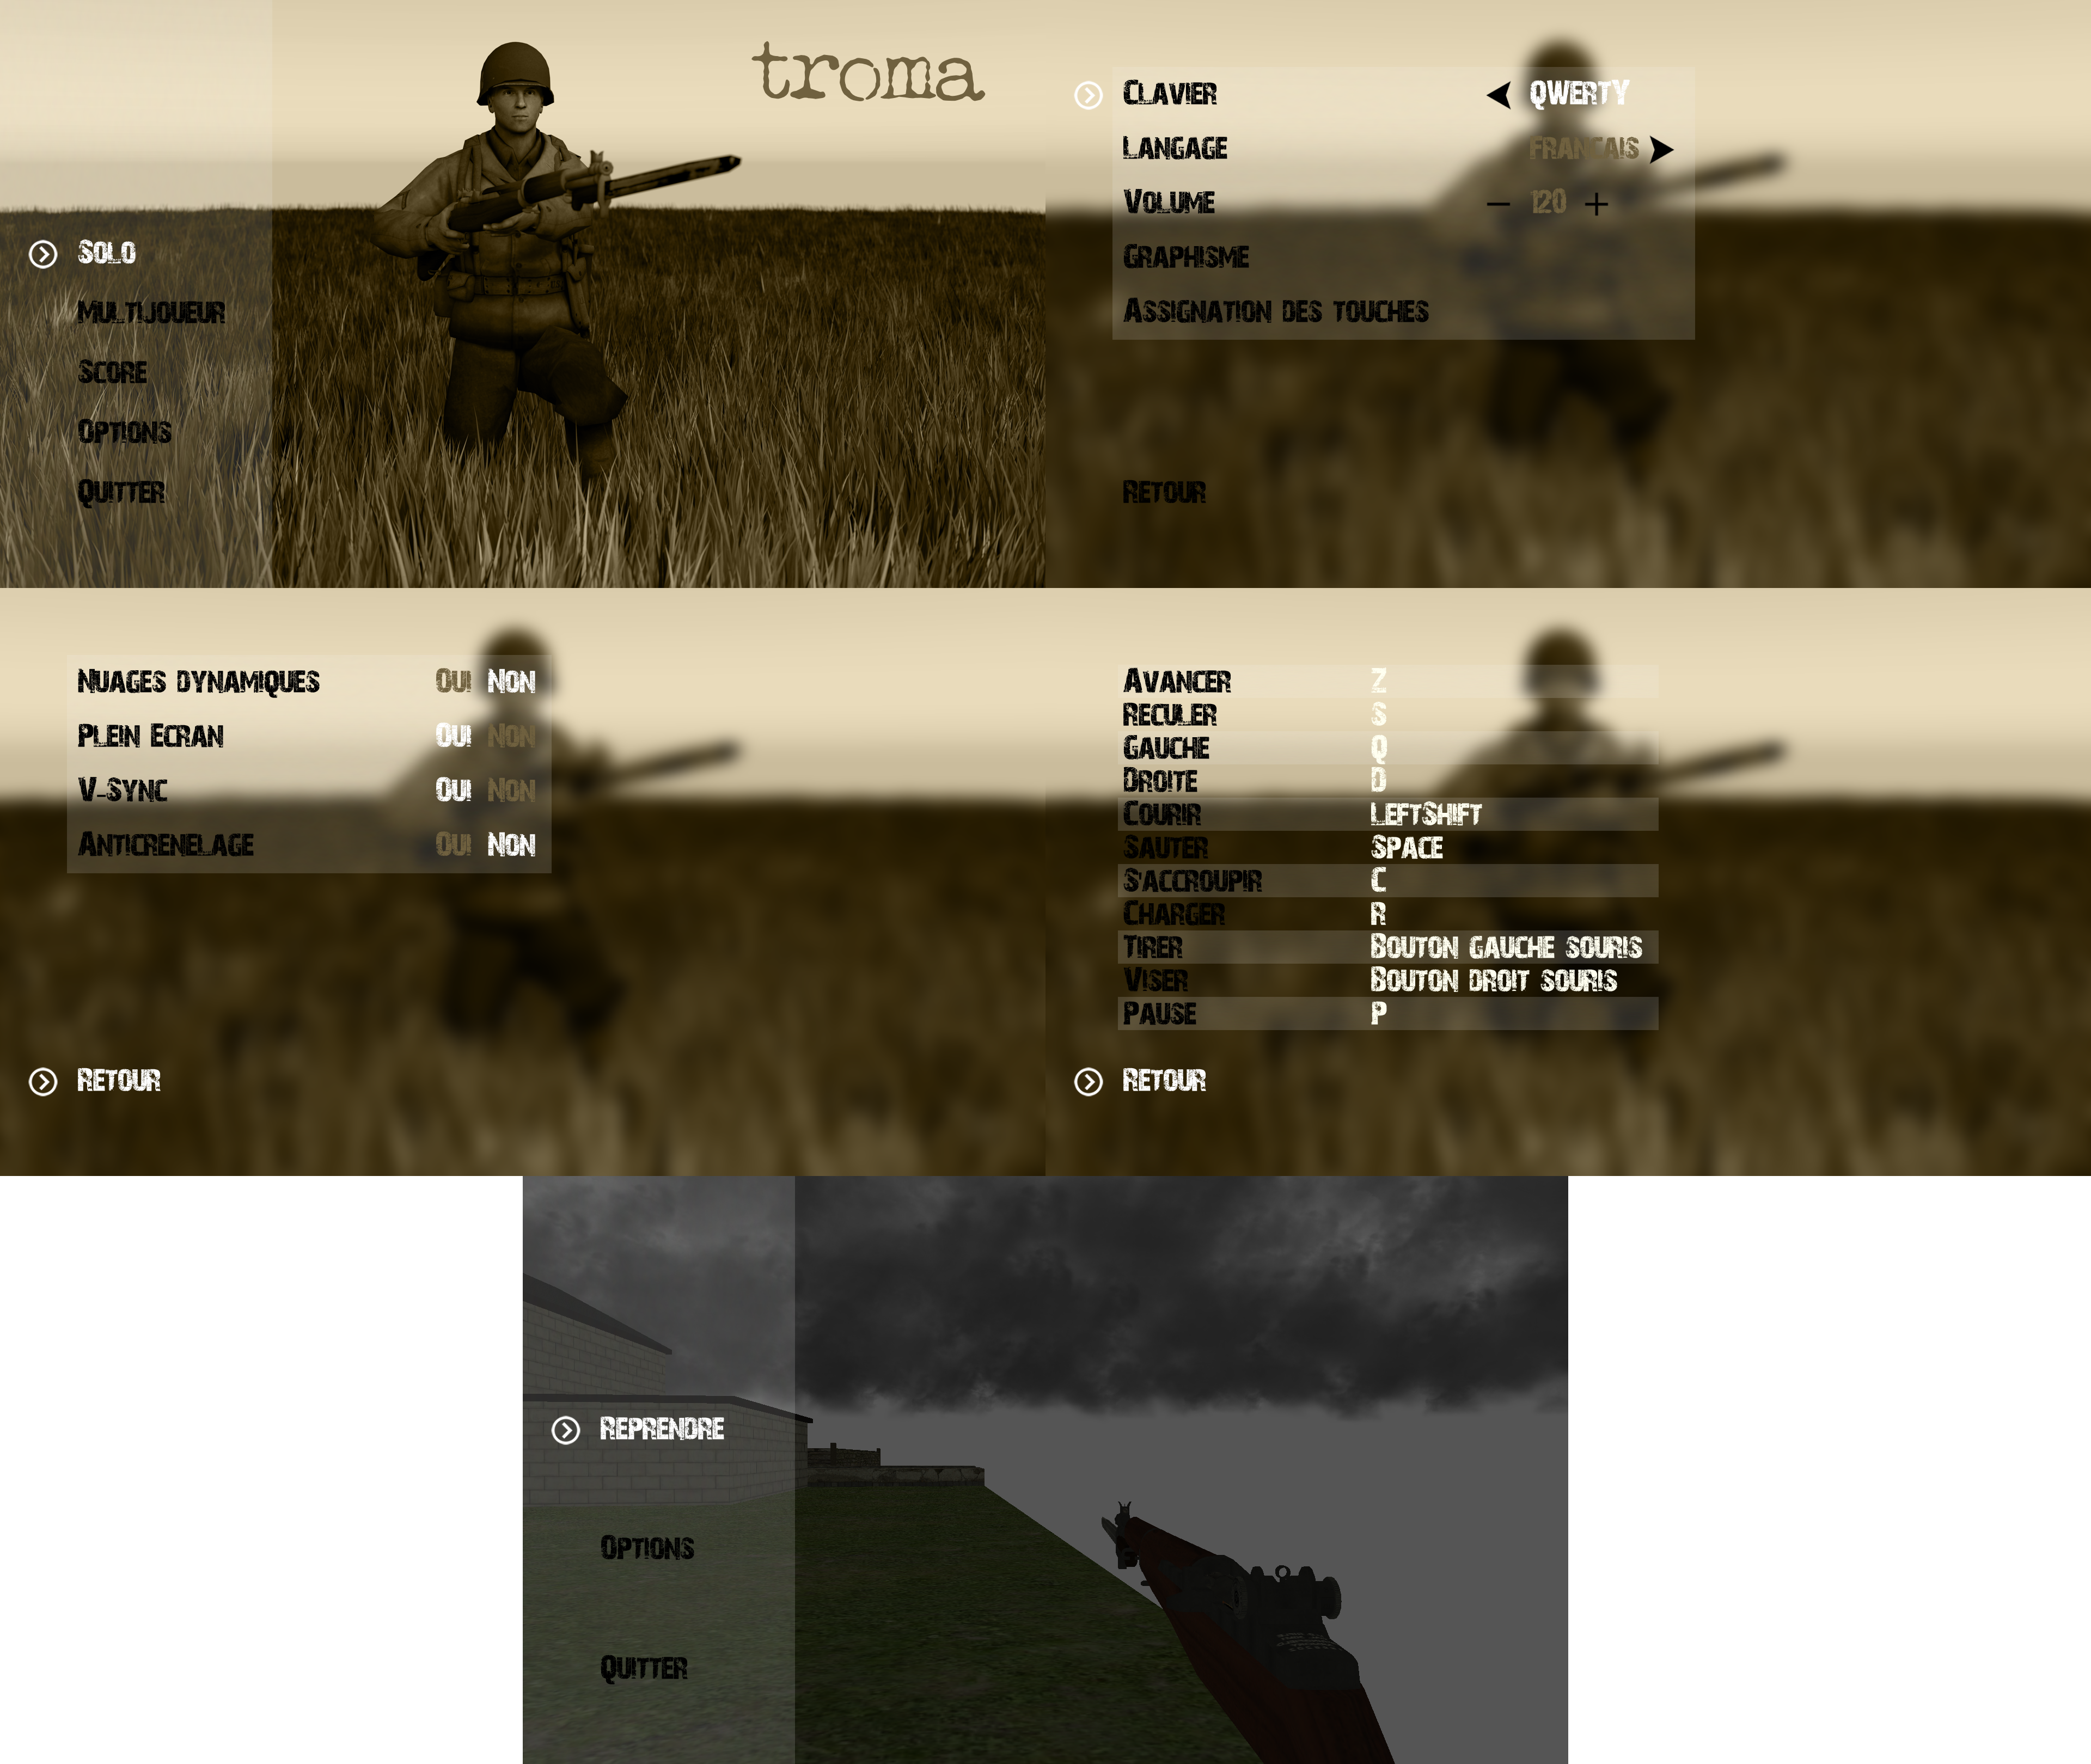
\includegraphics[width=11cm]{menu-3.png}
\caption{Captures d'écran de plusieurs menus à la fin du projet}
\end{figure}

Le design retenu suit la tendance actuelle dans le monde du jeu vidéo. C'est à dire un menu épurer, très sobre et s'accordant parfaitement avec notre jeu. L'idée principale repose sur un fond d'écran mettant en scène notre personnage 3D ainsi que son arme, des bandes blanches semi-transparentes ainsi l'application de flou gaussien.

Pour compléter cette interface, nous avons rajouté un écran de chargement qui évite à l'utilisateur d'avoir des ralentissements au lancement du jeu.

\section{Vidéos d'introduction}

Notre projet étant un jeu de guerre, nous voulions pouvoir informer les utilisateurs, dès le lancement du jeu, d'un âge conseillé. Ainsi nous avons choisi d'utiliser les logo de la l'agence PEGI\footnote{Pan European Game Information} dans une très courte vidéo avertissant les joueurs au lancement du jeu.

\begin{figure}[htbp]
\centering
\includegraphics[width=8cm]{pegi18.png}
\caption{Capture d'écran du PEGI 18}
\end{figure}

Pour compléter le démarrage de notre jeu, nous avons mis à profit nos différents talents artistiques pour réaliser, avec blender, une vidéo d'introduction de notre studio. Cette vidéo devait être courte et marqué les esprits.

Le fil conducteur de cette introduction est une grenade qui explose au ralenti. La caméra change régulièrement d'angle de vue jusqu'à revenir à sa position initiale. A ce moment là, l'explosion reprends à sa vitesse normale et on voit apparaître le texte ``Emagine Studio''.

\begin{figure}[htbp]
\centering
\includegraphics[width=11cm]{anim-eie.png}
\caption{Ensemble de captures d'écran de l'animation}
\end{figure}

Grâce à ces petits ajouts au lancement du jeu, nous sommes passés d’un jeu amateur à un jeu s'approchant au maximum de ceux sur le marché.

\section{HUD}

TODO: interface dans le jeux

\chapter{Audio}

\chapter{Gameplay}

\chapter{Réseau}

\chapter{Site web}

\chapter{Synthèses personnelles}

\section{Thibault}

\section{Rémy}

Novice dans le domaine de l'informatique, je pense que le projet est un bon moyen de s'améliorer en programmation. Durant ce projet, j'ai été en charge du son, du menu, du gameplay ainsi que du site web. Je ne suis pas le programmeur fou mais je me débrouille à ma manière pour réussir à faire avancer le projet.

C’est un groupe très dynamique où chaque personne du groupe s’entend avec les autres, j’ai bien aimé cet aspect la car on peut observer que dans certains autres groupes, l’égo de chacun prend le dessus et cela peut vite devenir l’anarchie.

Nous nous sommes très bien répartis les tâches. Les personnes qui savent le mieux codé font de la programmation un peu plus poussé, complexe (surtout Thibault Deutsch qui a un très bon niveau en programmation) pour permettre d’avoir un meilleur rendu visuel (tel que les particules pour les nuages où nous sommes tous restés bouche bée devant ce qu’il a fait). Ce qui nous permet aussi d’apprendre en regardant ce qu’il fait.

Chaque personne à son mot à dire et nous demandons l’avis du groupe pour soit supprimer ou garder quelque chose dans le projet. Si il y a toujours conflit, nous nous sommes mis d’accord au début d’année que ce soit le chef de projet qui tranche sur le sujet. Ce qui rend un peu plus notre projet comme une start up avec toutes les personnes du projet qui travail mais une personne qui a une part de responsabilité en plus.
Nous avons eu des problèmes tout au long du projet avec des parties qui ne s’implémentaient pas et qu’on devait absolument résoudre avant les soutenances. Des moments de stress plus intense que d’habitude qui ne nous aide pas beaucoup à l’avance du projet.

J’ai rencontré des difficultés sur certaine de mes parties, non pas parce que je ne savais pas comment faire, parce que je ne connaissais pas le langage approprié car je ne l’avais pas appris. Il a donc fallu aller se documenter sur internet et faire quelques exercices pratiques pour essayer de comprendre et de voir comment cela fonctionne.

J’ai beaucoup appris grâce à ce projet, que ce soit le travail en groupe, la répartition des tâches ou même d’avoir un projet à rendre comme en entreprises. Par rapport au travail en groupe je dois dire que c’est une très bonne chose de l’avoir expérimenté car dans beaucoup d‘entreprise, plusieurs personnes sont réunis sur un même projet. Ce qui signifie qu’une personne ne fait pas le projet seul, ils doivent se répartir les rôles, les tâches, qui fait quoi, et cela est très enrichissant car ce n’est pas si simple que cela quand tout est mal organisé dès le début. On doit surtout se comprendre entre nous, car l’incompréhension amène souvent les personnes à faire quelque chose qui n’était pas prévu par le groupe ou qui était déjà fait par quelqu’un d’autre et cela joue beaucoup sur le planning. On ne travaille pas tous en même temps donc il faut souvent faire des réunions ou se briefer pour voir qui est dans les temps sur ses parties ou non. J’ai bien aimé le fait qu’on puisse s’entraider mutuellement, si j’ai un problème sur une partie je peux demander à quelqu’un du groupe comment il aurait fait pour résoudre ce problème car on n’a pas tous la même vision des choses, et la plupart du temps cela fonctionne car la personne a pris le problème sous un autre angle.

Le projet m’a vraiment appris beaucoup que ce soit en termes de travail en groupe, ou en apprentissage personnel en programmation. Il m’a permis de respecter un planning et de ne pas reporter ce que j’avais à faire au lendemain pour ne pas retarder le groupe, car les parties sont liées entre-elles et cela entrainerait un retard pour le tout le groupe. 


\section{Marc}

Passionné d’informatique depuis mon enfance, j’ai toujours souhaité comprendre le fonctionnement d’un ordinateur ; aussi bien du côté matériel que logiciel. Le projet à réaliser en première année à l’EPITA m’a permis de répondre à ce besoin.

La conception d’un logiciel, en l’occurrence d’un jeu est une façon très stimulante pour apprendre et comprendre la programmation. La motivation pour mener à bien ce projet m’a permis d’acquérir une aisance vis-à-vis de la programmation orientée objet, mais aussi une nouvelle expérience de travail en groupe.

L’organisation que nous avons choisie fut de répartir différentes parties à un ou plusieurs membres afin de permettre une avancé rapide. Cependant nous avons eu l’occasion d’apporter aide, avis ou conseil aux autres membres.  Je me suis principalement occupé de la partie graphique et du réseau. En dehors de la programmation en elle-même, j’ai beaucoup appris sur la conception et le rendu d’objet en 3 dimensions en informatique, mais aussi sur la structure des réseaux et leur fonctionnement. Les difficultés majeures que j’ai rencontrées concernaient l’export des modèles et leur utilisation dans XNA. Heureusement j’ai pu trouver de l’aide soit sur des forums ou dans la documentation officielle soit auprès d’autres étudiants au sein du groupe ou de l’école. Les nombreux problèmes que nous avons pu rencontrer nous ont parfois démoralisé mais jamais découragé et nous avons toujours réussi à trouver des solutions. C’est ce que je retiens de cette expérience : ``Un problème sans solution est un problème mal posé'', Albert Einstein.

Concernant le groupe, nous avons su travailler en équipe et nous entraider. Je garde un bon souvenir de cette expérience qui m’a beaucoup apportée. Elle est indispensable pour une future insertion dans le milieu professionnel où savoir travailler en groupe est primordial.

Ce projet est le plus long et le plus élaboré que j’ai à mon actif mais c’est surtout le premier que j’ai réalisé en groupe. Il est le premier d’une longue série et m’a convaincu que j’avais fait le bon choix en venant à l’EPITA. En association des cours plus théoriques, les TP et les projets que nous avons à réaliser nous offrent une véritable expérience informatique. Bien que je n’ai pas vocation à travailler dans le domaine vidéo-ludique, j’ai beaucoup apprécié ces 6 mois de développement.

\section{Anthony}

L'idée de partir de zéro et de tout construire soit même m'a toujours beaucoup plu ainsi depuis le début je suis très motivé par ce projet non seulement car il s'agit de créer mon premier jeu mais également car je pense que nous pouvons aboutir à quelque chose de très convaincant.

Dans un premier temps j'ai vu ce projet comme un moyen d'apprendre à mener à bien une idée, de créer un produit. Cependant au fil du temps je me suis aperçu qu'il s'agissait de beaucoup plus que ça. La première chose qu'il faut savoir gérer, et à laquelle je n'avais pas forcement pensé au début est le travail en groupe, non seulement pour le chef de projet mais également pour le reste de l'équipe. Et cela nous amène directement au second point: la gestion du temps.

Je me suis rendu compte que ces deux points étaient reliés lorsqu'il a fallu avancer rapidement et en peu de temps sur notre travail! Il est apparu clair que nous devions optimiser notre temps et chacun s'est mis à travailler conjointement sur une partie du jeu.

Ainsi la répartition des taches et le travail régulier sont devenu les deux clés pour mener à bien notre projet.

Enfin, plus personnellement ce projet m'a apporté des nombreuses connaissances en C\# et plus globalement en programmation. J'ai appris différentes ``techniques''  sur la mise en place d'un projet, de 3D, d'interface... ceci étant applicables à n'importe quel langage! Et je pense que c'est ça le plus important, il faut apprendre des choses qui nous servirons pour le futur car la forme a, certes, de l'importance mais le fond en a doublement!

\chapter*{Conclusion}

Le projet Troma a débuté en Janvier 2014, nous avions l'objectif de réaliser un jeu de guerre sous le thème de la Seconde Guerre Mondiale. Le groupe a été formé à partir de quatre étudiants en première année sans connaissance préalables particulières en langage C\#. Cependant nous avons décidé dès le début de donner notre maximum en choisissant un jeu en 3D muni d'un mode de jeu en ligne ! 

Durant toute la phase de développement nous avons essayé de garder cet état d'esprit qui est de toujours donner le maximum. Les notes que nous avons reçu aux deux premières soutenances nous ont encore plus motive à toujours continuer dans cette voie. Nous avons donc implémenter toutes les fonctionnalités du jeu une par une avec plus ou moins de difficulté mais sans jamais abandonner même quand cela s’avérait beaucoup plus difficile que prévu. L'aspect technique n'a pas été la seule difficulté, le cote organisationnel des soutenances et du planning à respecter pour l'équipe en a aussi été une! Notre point fort à été de ne jamais attendre le dernier moment et d'essayer de prendre le maximum d'avance possible sur note avancée lorsque cela était possible!

Aujourd'hui nous sommes fier d'avoir réussi à mener à bien notre projet de bout en bout. Nous espérons que nous pourrons appliquer ce que nous avons appris durant cette période dans le futur!

\newpage
\pagenumbering{Roman}
\part*{Annexes}

\newpage
\listoffigures

\newpage
\tableofcontents
 
\end{document}